\subsection{Performances des modèles}

On examine les performances de nos modèles suite aux recherches d'hyperparamètres effectuées. On calcule une première fois le score (comme expliqué en section 2) sur le jeu utilisé pour entraîner le modèle (résultats affichés en bleu), puis sur un jeu de donnée de validation qui n'a pas été utilisé pour l'entraînement (résultats affichés en orange). Évidemment, les scores de validation sont inférieurs aux scores d'entraînement.

De manière étonnante, nos résultats sont exceptionnellement bons pour presque tous nos modèles (excepté la classification naïve bayésienne et les processus gaussiens), avec des performances supérieures à 90\% sur les jeux de validation.\\

On en déduit ainsi qu'on n'a ni sur-apprentissage, ni sous-apprentissage sur ces 4 modèles. D'ailleyrs, aucun de ces 4 modèles ne semble vraiment se démarquer.\\

La classification naïve bayésienne présente une forte tendance à sur-évaluer. En effet, elle ne fait aucune erreur sur le jeu d'entraînement mais a un score très faible (inférieur à 50\%).\\

Enfin, les processus gaussien présentent une forte tendance à sous-évaluer. En effet, les erreurs d'entraînement de de validation sont très élevées (un score inférieur à 50\% dans les deux cas).\\

Les résultats des deux derniers modèles nous indiquent d'ailleurs que notre jeu de donnée ne se prête pas aux analyses et hypothèses gaussiennes.\\

\begin{figure}[h]
    \centering
    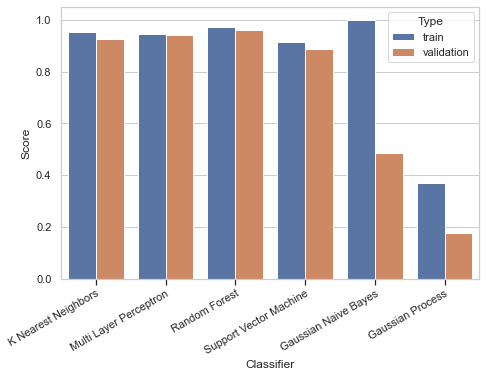
\includegraphics[scale=1]{Images/graphiques/results_barplot_V3.png}
    \caption{\it{Performances des modèles}}
    \label{fig:species_repartition}
\end{figure}